\documentclass{book}\usepackage{knitr}

% Preamble

%%%%%%%%%%%%%%%%%%%%%%
%% PACKAGES
%%%%%%%%%%%%%%%%%%%%%%
\usepackage[twoside,letterpaper,width=6in,height=8in]{geometry}
\usepackage{siunitx} % format units properly
\usepackage{wrapfig}
\usepackage[margin=10pt,font=small,labelfont=bf]{caption} % format captions
\usepackage{booktabs} % nicer tables
\usepackage{subcaption} 
\usepackage{csquotes} % block quotes
\usepackage{tikz}
\usepackage[inline, shortlabels]{enumitem} % inline enumeration
%\usepackage[version=4]{mhchem}
\usepackage{graphicx} % packages are used to modify the text and create bling.
%\includegraphics{{Home/CAMPUS/mwl04747/github/Environmnental-Sciences-in-East-Asia/images/}}
\usepackage{textcomp}
\usepackage{gensymb}
\usepackage{natbib}
\usepackage{glossaries}
\usepackage{amsmath}%
\usepackage{amsfonts}%
\usepackage{amssymb}%

%\usepackage[super,square,comma]{natbib}
%\usepackage{float}
%\usepackage{appendix}
%\usepackage{chngcntr}
%\usepackage{etoolbox}
%\usepackage[usenames]{xcolor}% for commenting in color!

\RequirePackage{hyperref} % For hyperlinked cross-references
\hypersetup{
    colorlinks,
    citecolor=blue,
    filecolor=blue,
    linkcolor=blue,
    urlcolor=blue
}


%----------------------------------------------------------
\newtheorem{theorem}{Theorem}
\newtheorem{acknowledgement}[theorem]{Acknowledgement}
\newtheorem{definition}[theorem]{Definition}
\newtheorem{example}[theorem]{Example}
\newtheorem{exercise}[theorem]{Exercise}

\newtheorem{problem}[theorem]{Problem}
\newtheorem{remark}[theorem]{Remark}
\newtheorem{solution}[theorem]{Solution}
\newtheorem{summary}[theorem]{Summary}
\newenvironment{proof}[1][Proof]{\textbf{#1.} }{\ \rule{0.5em}{0.5em}}
%----------------------------------------------------------

\AtBeginEnvironment{subappendices}{%
\chapter*{Appendix}
\addcontentsline{toc}{chapter}{Appendices}
%\counterwithin{figure}{section}
%\counterwithin{table}{section}
}

\makeatletter
\newcommand{\chapterauthor}[1]{%
  {\parindent0pt\vspace*{-25pt}%
  \linespread{1.1}\large\scshape#1%
  \par\nobreak\vspace*{35pt}}
  \@afterheading%
}
\makeatother

\renewcommand{\glstextformat}[1]{\textbf{\color{blue}\em #1}}

\newcommand{\R}{\mathbb{R}}
\newcommand{\carbondioxide}{CO$_2$~}



\title{Environmental Issues in East Asia}
\author{EA30e Spring 2021}
\date{\today}
\IfFileExists{upquote.sty}{\usepackage{upquote}}{}
\begin{document}

\maketitle
\makeglossaries

\frontmatter
\tableofcontents


\chapter*{Preface}

\section{Guiding Principles}

Environmental issues in East Asia are not unique or particularly more prevasive than other parts of the world. However, the issues are born from particular histories that may contrast with other parts of the world and other parts of the world may be able to learn from. 

In this project, the students in EA030e (Spring 2021) have written a textbook that highlights examples of environmental processes. Each student contributed to one theme, composed of two examples that highlight environmental issues of East Asia. 

\subsection{Context and Positionality}

As students in a college course located in Southern California, we approach the project with...


Our goal is not to call out environmental issues in East Asia, but to point to linkages of how a range of globalized economy contribute to these environmental problems. 

In the end, it would be useful for us to acknowledge we have some capacity to address these how these global linkages could be modified to reduce these environmental issues.

We are not experts, but learning... if there are errors please let us know... We recommend that suggestions be submitted via a github pull request.

\subsection{Goals}

Processes across horizontal boundaries define many environmental patterns that frame human interactions with the environment. How do humans impact processes that cross these boundaries and how do humans influence these ecosystem interface?

\subsection{Rationale}

We hope to learn more about the how environmental issues are expressed in different parts of the world and to what extent can we learn from this work. 

\subsection{Activity}

Each group will be composed of two students, that will become experts and teach their classmates on the topic. 

\section{East Asia and the World}







\section{Acknowledgments}

Everyone in the world!




\chapter{Author Guide}\label{ch:guide}

\subsection*{Why Learn \LaTeX?}

\subsection*{How to Learn \LaTeX?}


\subsubsection{R Chunks}

To create effective graphics, each chapter will have a rchunk that creates a graphic for the chapter. To review and learn R, here are some resources: 

\begin{itemize}
  \item \href{www.tbd.com}{Marc's Video Description}
  \item \href{https://rmd4sci.njtierney.com/}{RMarkdown for Scientists (super helpful!)}
  \item \href{https://rmarkdown.rstudio.com/lesson-1.html}{R Studio Tutorial}
  \item \href{https://rstudio.com/wp-content/uploads/2016/03/rmarkdown-cheatsheet-2.0.pdf?_ga=2.107420162.161662097.1613074083-214354297.1613074083}{R Studio's Cheatsheet}
  \item \href{https://bookdown.org/yihui/rmarkdown-cookbook}{R Markdown Cookbook -- Robust Source}
\end{itemize}


\subsection*{Noting Your Contribution}

Because this is an ongoing project, you should record your contribution to each chapter -- but also let go of these contributions at some point; Others might revise and their authorship might take some precedence, so you should both invest in the product but also be willing to detach from the final outcome as others contribute. This will feel uncomfortable at times, but please note from the beginning this is a social process and as such subject to negotiation. Please be generous to the authors that laid the foundation and be respectful of those that follow. 

\section{Setting Up Book Project--Type Setting w/ \LaTeX}

\subsection*{Latex Book Class}

Currently, the text is written using the standard book class. %However, in 2019, I (Los Huertos) will convert the format to a Tufte book class. 

\subsection*{Structuring the Text with Nested Hierarchies}

Contributors divide their contributions into sections and subsections. This format allows a consistent approach to structuring the text and forcing themes to be organized in blocks that can be used to organize the overall text. We use section, subsection, and subsubsection to break up the topic into bite sizes. 

To accomplish this, contributors use the \verb"\section{Section}" command for major sections, and the \verb"\subsection{Subsection}" command for subsections, and a similar approach for subsubsections. 

NOTE: for each nested level, it MUST be followed by the lowest level in the section before a paragraph is started -- in contrast to what is shown above!

NOTE: We may dispense with subsubsections in the future to provide a less blocky structure, but for now they remain useful. 

\subsection*{Font Changes}

We can use various methods to alter the typeset: \emph{Emphasize}, \textbf{Bold}, \textit{Italics}, and \textsl{Slanted}. We can also typeset \textrm{Roman}, \textsf{Sans Serif}, \textsc{Small Caps}, and \texttt{Typewriter} texts.  Look online to see the commands to accomplish these changes. 

You can also apply the special, mathematics only commands $\mathbb{BLACKBOARD}$, $\mathbb{BOLD}$, $\mathcal{CALLIGRAPHIC}$, and $\mathfrak{fraktur}$. Note that blackboard bold and calligraphic are correct only when applied to uppercase letters A through Z.

You can apply the size tags -- Format menu, Font size submenu -- {\tiny tiny}, {\scriptsize scriptsize}, {\footnotesize footnotesize}, {\small small}, {\normalsize normalsize}, {\large large}, {\Large Large}, {\LARGE LARGE}, {\huge huge} and {\Huge Huge}.

You can use the \verb"\begin{quote} etc. \end{quote}" environment for typesetting short quotations. Select the text then click on Insert, Quotations, Short Quotations:

\begin{quote}
The buck stops here. \emph{Harry Truman}

Ask not what your country can do for you; ask what you can do for your
country. \emph{John F Kennedy}

I am not a crook. \emph{Richard Nixon}

I did not have sexual relations with that woman, Miss Lewinsky. \emph{Bill Clinton}
\end{quote}

The Quotation environment is used for quotations of more than one paragraph. Following is the beginning of description of \LaTeX from \emph{Wikipedia}:

\begin{quotation}
LaTeX (/ˈlɑːtɛx/ LAH-tekh or /ˈleɪtɛx/ LAY-tekh, often stylized as \LaTeX) is a software system for document preparation. When writing, the writer uses plain text as opposed to the formatted text found in ``What You See Is What You Get'' word processors like Microsoft Word, LibreOffice Writer and Apple Pages. The writer uses markup tagging conventions to define the general structure of a document (such as article, book, and letter), to stylise text throughout a document (such as bold and italics), and to add citations and cross-references. A \TeX distribution such as \TeX Live or MiK\TeX is used to produce an output file (such as PDF or DVI) suitable for printing or digital distribution.

LaTeX is widely used in academia for the communication and publication of scientific documents in many fields, including mathematics, statistics, computer science, engineering, physics, economics, linguistics, quantitative psychology, philosophy, and political science. It also has a prominent role in the preparation and publication of books and articles that contain complex multilingual materials, such as Sanskrit and Greek. \LaTeX uses the TeX typesetting program for formatting its output, and is itself written in the TeX macro language.''
\end{quotation}

Use the Verbatim environment if you want \LaTeX\ to preserve spacing, perhaps when
including a fragment from a program such as:
\begin{verbatim}
#include <iostream>         // < > is used for standard libraries.
void main(void)             // ''main'' method always called first.
{
 cout << ''This is a message.'';
                            // Send to output stream.
}
\end{verbatim}
(After selecting the text click on Insert, Code Environments, Code.)


\subsection*{Mathematics and Text}

\subsubsection{Warning: Special Characters}

When you use percent and ampersand symbols, hash tags, and other non-standard ASCII characters, \LaTeX will be very uncooperative. So, do yourself a favor and make sure you understand that these are used for special typesetting functions. To use them you have to ``escape'' and use commands to get them to do what you might usually expect!  \% \# \& \`e \~n `` and '' to show a few that do not reflect the key stroke you might expect. 

\LaTeX doesn't like a range of characters or they reserved for special behavior...

For example, the \# is used for tabs in a table environment. \% is used to make comments, thus stuff behind a \% is ignored. There are lots of others, but these come up the most.

\subsubsection{Creating equations}

One of the most powerful parts of \LaTeX is how it can be used to write complex equations, with all those symbols and Greek letters! This can be done inline $y = mx + b + \epsilon$ for fairly simple equations, or set apart for more complex equations:

\begin{equation}
\int_0^\infty e^{-x^2} dx=\frac{\sqrt{\pi}}{2}
\end{equation}

\subsubsection{Theorems, etc}
\begin{theorem}
(The Currant minimax principle.) Let $T$ be completely continuous selfadjoint operator
in a Hilbert space $H$. Let $n$ be an arbitrary integer and let $u_1,\ldots,u_{n-1}$ be
an arbitrary system of $n-1$ linearly independent elements of $H$. Denote
\begin{equation}
\max_{\substack{v\in H, v\neq
0\\(v,u_1)=0,\ldots,(v,u_n)=0}}\frac{(Tv,v)}{(v,v)}=m(u_1,\ldots, u_{n-1})
\label{eqn10}
\end{equation}
Then the $n$-th eigenvalue of $T$ is equal to the minimum of these maxima, when
minimizing over all linearly independent systems $u_1,\ldots u_{n-1}$ in $H$,
\begin{equation}
\mu_n = \min_{\substack{u_1,\ldots, u_{n-1}\in H}} m(u_1,\ldots, u_{n-1}) \label{eqn20}
\end{equation}
\end{theorem}
The above equations are automatically numbered as equation (\ref{eqn10}) and
(\ref{eqn20}).


\subsection{Lists Environments: Making bulletted, numbered, description lists}

We use special commands to create an itemized list.

You can create numbered, bulleted, and description lists
(Use the Itemization or Enumeration buttons, or click on the Insert menu
then chose an item from the Enumeration submenu):

\begin{enumerate}
\item List item 1

\item List item 2

\begin{enumerate}
\item A list item under a list item.

\item Just another list item under a list item.

\begin{enumerate}
\item Third level list item under a list item.

\begin{enumerate}
\item Fourth and final level of list items allowed.
\end{enumerate}
\end{enumerate}
\end{enumerate}
\end{enumerate}

\begin{itemize}
\item Bullet item 1

\item Bullet item 2

\begin{itemize}
\item Second level bullet item.

\begin{itemize}
\item Third level bullet item.

\begin{itemize}
\item Fourth (and final) level bullet item.
\end{itemize}
\end{itemize}
\end{itemize}
\end{itemize}

\begin{description}
\item[Description List] Each description list item has a term followed by the
description of that term.

\item[Bunyip] Mythical beast of Australian Aboriginal legends.
\end{description}

\subsection{Theorem-Like Environments}

The following theorem-like environments (in alphabetical order) are available
in this style.

%\begin{acknowledgement}
%This is an acknowledgement
%\end{acknowledgement}

\begin{example}
This is an example
\end{example}

\begin{exercise}
This is an exercise
\end{exercise}


%\begin{proof}
%This is the proof of the lemma.
%\end{proof}

%\begin{notation}
%This is notation
%\end{notation}

%\begin{problem}
%This is a problem
%\end{problem}

%\begin{proposition}
%This is a proposition
%\end{proposition}

%\begin{remark}
%This is a remark
%\end{remark}

%\begin{summary}
%This is a summary
%\end{summary}

\begin{theorem}
This is a theorem
\end{theorem}

%\begin{proof}
%[Proof of the Main Theorem]This is the proof.
%\end{proof}

%\subsubsection{``Child'' Rnw Contributions}

%This is a chapter that we can input into the text... you will each create a chapter without the preamble and begin and end document... that can be integrated into a single book! 

\subsection{Peer Review Commenting}

You can put your comments in square brackets and in color for things that need help. \textcolor{red}{[This section is confusing, I am not sure what commenting means.]}

\subsection{Adding Figures, etc}

\subsubsection{Using Rnw Files}

To generate R figures, we use R chunks in and Rnw file, where the text is integreated. When we compile into a PDF, the program converts the files into TeX files and then combineds them into a single pdf. 

For each chapter, we create a ``child'' document and Marc will help you create that text when you begin. 

\subsubsection{Creating a floating figure}

This is my floating figure (Figure \ref{fig:plot}).

\begin{figure}

\caption{My plot's caption is here!}
\label{fig:plot}
\end{figure}

\subsubsection{Using R to Create Effective Figures}

R Markdown can be a very powerful tool to integrate R code, figures and text. Making high quality figures that are both clear and aestically pleasing will be something that we need to think about it. 

\begin{itemize}
  \item Axis Labels -- Labelled with clarity 
  \item Axis Text -- Size, Orientation 
  \item Captions (usually better than titles)
  \item References connecting labels to references
  \item ADA accessible (e.g. color impairment mitigation)
\end{itemize}

For example, here's code to generate a pretty good figure: 



\begin{knitrout}
\definecolor{shadecolor}{rgb}{0.969, 0.969, 0.969}\color{fgcolor}\begin{kframe}


{\ttfamily\noindent\bfseries\color{errorcolor}{\#\# Error in file(file, "{}rt"{}): cannot open the connection}}

{\ttfamily\noindent\bfseries\color{errorcolor}{\#\# Error: package or namespace load failed for 'tidyverse' in loadNamespace(i, c(lib.loc, .libPaths()), versionCheck = vI[[i]]):\\\#\#\ \ namespace 'dplyr' 0.8.5 is already loaded, but >= 1.0.0 is required}}

{\ttfamily\noindent\bfseries\color{errorcolor}{\#\# Error in createDataPartition(., p = 0.8, list = FALSE): object 'maunaloa' not found}}

{\ttfamily\noindent\bfseries\color{errorcolor}{\#\# Error in eval(expr, envir, enclos): object 'maunaloa' not found}}

{\ttfamily\noindent\bfseries\color{errorcolor}{\#\# Error in eval(expr, envir, enclos): object 'maunaloa' not found}}

{\ttfamily\noindent\bfseries\color{errorcolor}{\#\# Error in eval(expr, envir, enclos): object 'maunaloa' not found}}

{\ttfamily\noindent\bfseries\color{errorcolor}{\#\# Error in is.data.frame(data): object 'maunaloa' not found}}

{\ttfamily\noindent\bfseries\color{errorcolor}{\#\# Error in summary(model): object 'model' not found}}

{\ttfamily\noindent\bfseries\color{errorcolor}{\#\# Error in predict(., test.data): object 'model' not found}}

{\ttfamily\noindent\bfseries\color{errorcolor}{\#\# Error in mean((pred - obs)\textasciicircum{}2, na.rm = na.rm): object 'predictions' not found}}\end{kframe}
\end{knitrout}

In the case of Figure \ref(fig:maunaloa), we can a create a figure that has all of the characteristics listed above, except perhaps ADA. Creating a "alt text" for the figure is something we might want to consider. 

\begin{figure}
\begin{knitrout}
\definecolor{shadecolor}{rgb}{0.969, 0.969, 0.969}\color{fgcolor}\begin{kframe}


{\ttfamily\noindent\bfseries\color{errorcolor}{\#\# Error in ggplot(train.data, aes(decimal.date, average)): object 'train.data' not found}}\end{kframe}
\end{knitrout}
\caption{Carbon Dioxide Concentrations (Mauna Loa, HI). Source: Scripps/NOAA.}
\label{fig:co2-graphic}
\end{figure}

\subsection{Using Boxes}

\fbox{
\begin{minipage}[c]{.9\textwidth}
\subsection{minibox X}

Some text
\end{minipage}
}

\subsection{ Cross-References, Citations, and Glossaries}

\subsubsection{Cross-References}

We can cross-reference sections (e.g. Section~\ref{ch:critical-zone}  or figures (Figure~\ref{fig:maunaloa}) using several methods. I suggest you look at the this Rmd file to see how I did it in these examples.

You can also create links to URLs or hyperlinks, e.g. \url{http://texblog.org}. However, if these addresses change, then the link will break, so I suggest you only link to internal references.

\subsubsection{Bibliography generation}

There will be two steps to cite our sources. First, we need to add the reference to a database, or bib file. This is titled 'References.bib' and is located in the main folder in our respository. When you add information to the bib file, be sure to paste in the reference using a bibTeX format. 

Second, we'll need to place in-line citations, using \verb"\citep{knitr}", which produces \citep{knitr}, by using a key, which is knitr in this case. 

For example, you might write, ``This document was produced in RStudio using the knitr package (\citep{knitr}). Also try \verb"\citet{LosHuertos2017OverviewR}" to create use the author name as the subject: \citet{LosHuertos2017OverviewR} wrote an guide to help students learn R. 

Note: You will see these citations automatically put in alphabetic order in the Bibliography at the end of the PDF. 

%Currently, we are using the ecology.bst, but it has trouble with misc type of references, so I will changing this in 2019. 

\subsubsection{Creating glossary words}
 
\newglossaryentry{peat}{
	name=peat, 
	description={is cool.}
}

\begin{definition}
This is a definition and the word is use in an glossary, e.g. \gls{peat}. \Gls{peat} is when you want to capitalize the defined word without having to re-define a capitalized version, the only downside of case sensitivity in \LaTeX.
\end{definition}


\chapter{Chapter Title}

\chapterauthor{Chapter Author Name}\footnote{Statement of Contributions-- For example, ``The chapter was first drafted by Marc Los Huertos (2021). The author recieved valuable feedback from X, and Y and Z to improve the chapter. Slater revised the chapter in 2022 with suggestions from Cater.'' Note: I am still working on the formatting for this to improve it.}

\section{Section Heading}% Avoid putting text between section and subsection headings.

\subsection{Subsection Headings} % Avoid putting text between subsection and subsubsection headings. Not applicable if you don't have subsections!

Some text here... if you cut and paste, be sure to make sure you don't include formatted characters outside the ASCII values. See Author Guide\ref{ch:guide}.

\subsubsection{Optional Subsubsection Headings} % Again try to avoid putting text between the subheadig and the subsubheading to main a structural consistency.

some text here....

\section{Goals of this template}

This template will NOT teach you how to use \LaTeX! To accomplish that, we'll rely on some great online resources that you can find on in Chapter \ref{ch:guide}. 

Instead this section of the document is designed to demonstrate how our textbook will look, feel, and ultimately how we contribute to the project.

This document also compiles all of our projects into a single PDF, where each chapter is composed of a input tex file.

\section{Here's figure}

\subsection{R Created Figures}

First we create an R chunk and add some code. In this case, I created a floating figure which can be referenced (Figure~\ref{fig:pressure})!  

\begin{figure}
\begin{knitrout}
\definecolor{shadecolor}{rgb}{0.969, 0.969, 0.969}\color{fgcolor}\begin{kframe}
\begin{alltt}
\hlkwd{plot}\hlstd{(pressure)}
\end{alltt}
\end{kframe}
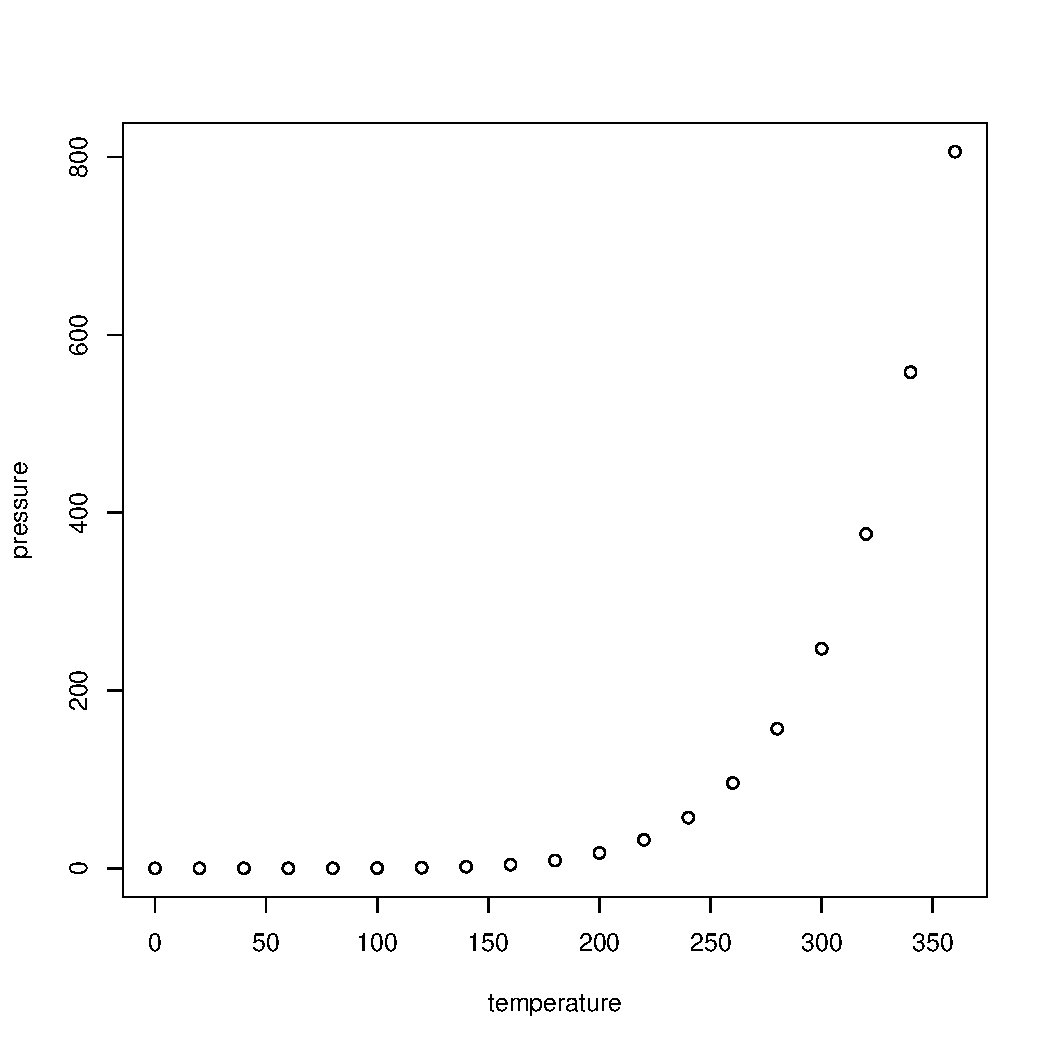
\includegraphics[width=\maxwidth]{figure/fig:pressure-1} 

\end{knitrout}
\caption{Figure Caption...we should turn "echo=False" in the R chunk options, but I left it true for now. (source: ??)} % define the caption, then the label.
\label{fig:pressure}

\end{figure}

\subsection{Imported Figures}

All figures and images that are imported should be put into the "images" sudirectory to keep stuff organized. Even better to create a subdirectory with your images, but we can naviagate as we go.

Figure \ref{fig:vadose} is a good example of this.

\begin{figure}
\includegraphics[width=\linewidth]{images/Lee-Vadose}
\caption{Vadose zone is neato (Source: \citet{lee2017fifty}).}
\label{fig:vadose}
\end{figure}

In this case, I had to specify the width so it would fit on the page!  See the Rnw file for the code. Notice, I was also abel to ``reference'' the figure in the text.
 

\chapter{Title...}

\chapterauthor{Nora}

some random change - nora tahbaz, NEW CHANGE
 getting ahead againo...3:08pm.

$\rightarrow$

\section{What the Polar Vortex and why do we care?}

\subsection{What Factors Drive Land Use Change?}




\mainmatter


\chapter{The Earth System}\label{earthsystem}

\chapterauthor{Marc Los Huertos}

\section{The Sun's Energy and the Earth's Temperature}

The temperture of the Earth's surface is the result of a balance -- the energy entering the atmosphere and the leaving the atmosphere. Most of this energy is in the form of light or electromagnetic radiation (Figure~\ref{fig:earthbudget}). 

\begin{figure}
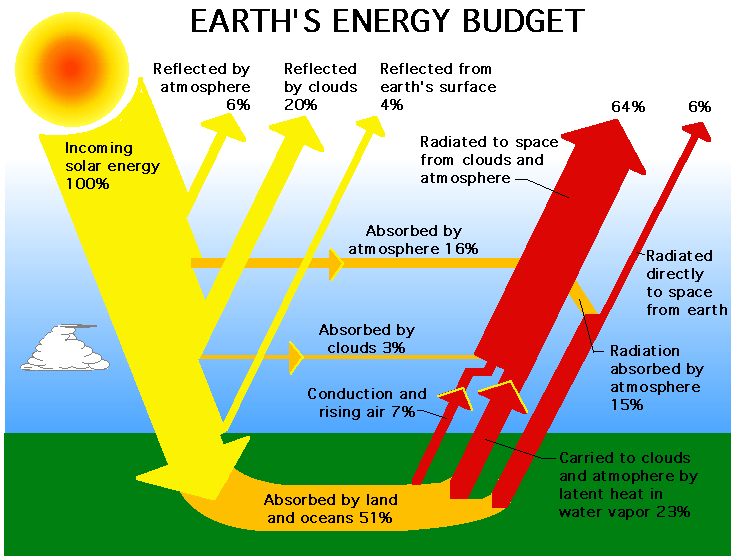
\includegraphics[width=\linewidth]{images/earth-system/earth-rad-budget-nasa-erbe.png}
\caption{caption}
\label{fig:earthbudget}
\end{figure}

Light enters the atmosphere, where some is absorbed and some is reflected. Light interacts in different ways with land, oceans, and vegetation, which is beyond the scope of our project. The ``quality'' of light changes through these processes. 

\subsection{The Spectrum of Light Entering and Exiting the Earth's Surface}

As the sun's electromagnetic radiation interacts with the Earth's Atmosphere, certain wavelengths are absorbed and filtered out (Figure~ \ref{fig:em-entering}).

\begin{figure}
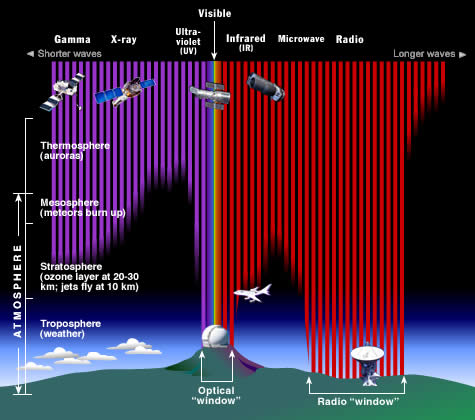
\includegraphics[width=\linewidth]{images/earth-system/em-radiation-atmosph-depth-stsci.jpg}
\caption{Various wavelengths of solar electromagnetic radiation penetrate Earth's atmosphere to various depths. Fortunately for us, all of the high energy X-rays and most UV is filtered out long before it reaches the ground. Much of the infrared radiation is also absorbed by our atmosphere far above our heads. Most radio waves do make it to the ground, along with a narrow `window' of IR, UV, and visible light frequencies. Source: STCI/JHU/NASA.}
\label{fig:em-entering}
\end{figure}

\subsection{The Atmosphere and Greenhouse Effect}



\section{Carbon Biogeochemistry}

\subsection{Long and Short Time Scales}

The carbon cycle processes occur at wide range of temporal scales from hundreds of millions of years to seasons of the year. These have been referred to as long and short carbon cycles. However, for our purposes, I will call them ``geologic carbon'' and ''biosphere carbon'' processes. 

\subsection{Rock Cycle and Geologic Carbon}

The carbon cycle describes changes in the fluxes and reservoirs of carbon in the Earth system. On very long time-scales, millions of years, the primary reservoirs of carbon are the atmosphere, ocean, and rocks (limestone). Carbon moves between these reservoirs through volcanic outgassing, silicate weathering, and limestone sedimentation. The carbon cycle is linked to Earth's energy balance through atmospheric carbon in the form of \carbondioxide, a greenhouse gas.

\subsubsection{Mountains and Erosion}

\ref{fig:carbonpools}

\begin{figure}
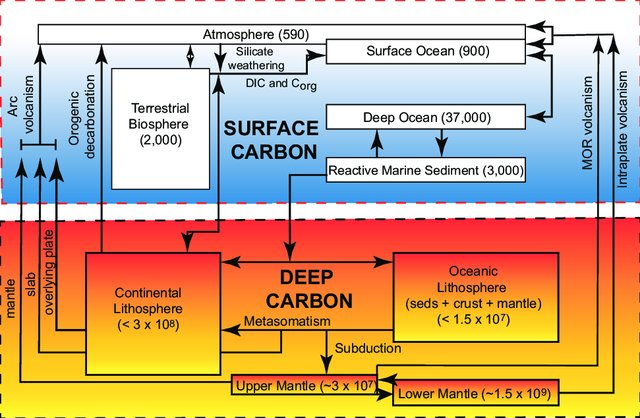
\includegraphics[width=\linewidth]{images/earth-system/Carbon-reservoirs-and-cycles-in-the-Earth.jpg}
\caption{Carbon reservoirs and cycles in the Earth. The figure shows short-and long-term cycles; biosphere and geologic carbon reservoirs and fluxes, and the relative sizes and residence times (y axis) of respective carbon. Numbers in brackets refer to the total mass of carbon in a given reservoir, in Pg C (1Pg C = 10$^{15}$ g carbon). All reservoirs are pre-industrial. Abbreviations: C org = organic carbon; DIC = dissolved inorganic carbon; MOR = mid ocean ridge; seds = sedimentary rocks. Adapted from Lee et al. (2019 And references therein).}
\label{fig:carbonpools}
\end{figure}

\subsubsection{Subduction Burial and Carbon Recycling}

Figure~\ref{fig:longtermcarbon}

\begin{figure}
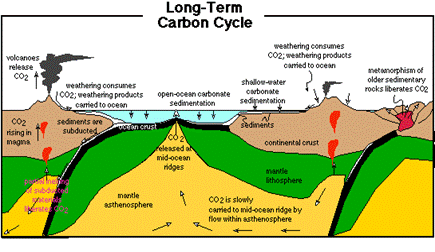
\includegraphics[width=\linewidth]{images/earth-system/long-term-carbon.png}
\caption{Schematic of the long-term carbon cycle (from Bice, 2001)}
\label{longtermcarbon}
\end{figure}

\subsection{Photosynthesis, Respiration, and Biosphere Carbon}

\subsubsection{Soil Respiration and the Soil Profile}

Carbon in soils is respired -- but different pools might have different rates of respiration. Sometimes these pools are distinquished as an active soil organic carbon pool and slow soil organic carbon pool. Although the reference of ``slow'' causes confusion with long-term, geologic carbon, but soil organic carbon remains a component of what we are refering to as biosphere carbon. 

The surface of the soil tends to have more SOC and microbes that can use that carbon for respiration. Lower down in the soil profile, we tend to see lower amounts of SOC and lower microbial biomass (Figure~\ref{fig:soilcarbon}. In addition, soils in the lower part of the profile tend to have more aggregation that protects SOC from microbial attack, thus a key area that soil carbon can seqeustor carbon. 

In addition to these microbial biomass and aggregate patterns, the microbes aree more senstive to temperature changes near the surface as measured by Q10 -- the rate of biochemical processes with a 10 degree C increase in temperature. Thus, soil processes, such as respiration, is likely to increase more near the surface with global warming that the lower part of the soil profile.  

\begin{figure}
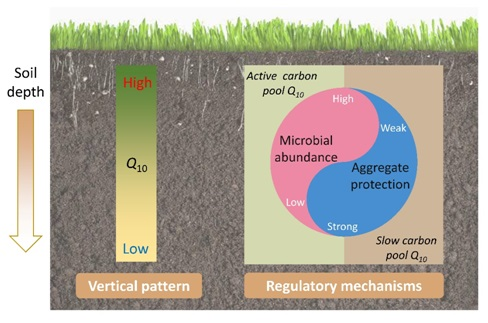
\includegraphics[width=\linewidth]{images/earth-system/Q10-SOC-Regulation.jpg}
\caption{Regulatory Mechanisms of the Temperature Sensitivity of Soil Organic Matter Decomposition in Alpine Grasslands (Source: \citet{Qineaau1218, CAS2021researchers}).}
\label{fig:Q10-SOC}
\end{figure}


\section{Fossil Fuels and Carbon Dioxide Trends}\label{sec:fossilfuels}

As part if the industrial revolution, our energy sources have put more \carbondioxide from the biosphere (soils and forests) and geologic carbon (coal, petroleum). 

\subsection{The Signal of Geologic and Biosphere Carbon in Atmosphere}

The combined contribution from geologic and biosphere carbon in the atmosphere is clearly documented from numerous sources. First, look at data collected at the Mauna Loa where \carbondioxide measurements have been taken continuously since the late 1950s. 

Figure~\ref{fig:maunaloa2}

\begin{figure}
\begin{knitrout}
\definecolor{shadecolor}{rgb}{0.969, 0.969, 0.969}\color{fgcolor}\begin{kframe}


{\ttfamily\noindent\bfseries\color{errorcolor}{\#\# Error in ggplot(train.data, aes(decimal.date, average)): object 'train.data' not found}}\end{kframe}
\end{knitrout}
\caption{Carbon Dioxide Measure on Mauna Loa, HI}
\label{fig:maunaloa2}
\end{figure}






\chapter{Monsoons and East Asia Climates}

\section{Temperature Gradients and Latitude}





\chapter{Critical Zone}\label{ch:critical-zone}

\chapterauthor{Marc Los Huertos}\footnote{The chapter was first drafted by Marc Los Huertos (2021). The author recieved valuable feedback from X, and Y and Z to improve the chapter.}

\section{What is the Critical Zone}

The crticical zone refers the the portion of the Earth's skin where the zone where rock meets life. The Critical Zone supports all terrestrial life.

The critical zone includes the following:

\begin{itemize}
  \item A permeable layer from the tops of the trees to the bottom of the groundwater;
  \item An environment where rock, soil, water, air, and living organisms interact and shape the Earth's surface;
  \item Water and atmospheric gases move through the porous Critical Zone, and living systems thrive in its surface and subsurface environments, shaped over time by biota, geology, and climate.
\end{itemize}

All this activity transforms rock and biomass into the central component of the Critical Zone - soil; it also creates one of the most heterogenous and complex regions on Earth.

Its complex interactions regulate the natural habitat and determine the availability of life-sustaining resources, such as food production and water quality.

These are but two of the many benefits or services provided by the Critical Zone. Such `Critical-Zone Services' expand upon the benefits provided by ecosystems to also include the coupled hydrologic, geochemical, and geomorphic processes that underpin those ecosystems.

\begin{figure}
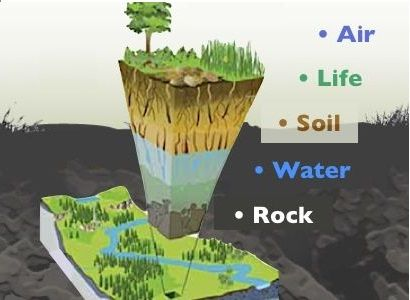
\includegraphics[width=\textwidth]{images/critical-zone/criticalzone.jpg}
\caption{The Critical Zone is an interdisciplinary field of research exploring the interactions among the land surface, vegetation, and water bodies, and extends through the pedosphere, unsaturated vadose zone, and saturated groundwater zone. Critical Zone science is the integration of Earth surface processes (such as landscape evolution, weathering, hydrology, geochemistry, and ecology) at multiple spatial and temporal scales and across anthropogenic gradients. These processes impact mass and energy exchange necessary for biomass productivity, chemical cycling, and water storage.}
\label{fig:criticalzone}
\end{figure}

\subsection{What are the environmental implications of the Critical Zone?}

The critical zone as a concept and as a material space pushes us to think of the porousity of the Earth's surface --- the gas and fluid flows through rocks, soils, and plants. We can begin to appreciate the complexity of the transport and fate of chemical pollutants as they enter the soil and become part of the vadose zone and perhaps the ground water table -- moving with water and diffusing through the water, simultaneously.

\section{Hydrologic Aspects}

\subsection{The Vadose Zone}

Jeji is a volcanic island is located some XX km south of the Korean Penisula. Water runs off the steep slopes quickly and water supplies are limited on the island. To adddress this...\citet{lee2017fifty}.

\begin{figure}
\includegraphics[width=\linewidth]{images/critical-zone/Lee-Vadose.png}
\caption{... (Source: \citep{lee2017fifty}).}
\label{fig:vadose2}
\end{figure}



\chapter{Land Use in East Asia}

What is Land Use Change?

What Factors Drive Land Use Change?

How Land Use Change is Measured and Quantified

Integration of sociology

with data science: spatial data compiled from aerial photos, Landsat satellite images, topographic maps, GPS data, etc.

Requires classification and division of land-space types

Ecological Effects of Land Use Change on Soil, Air, and Water

\section{Impacts on Soil}

Deforestation and soil degradation

lack of stability (erosion) and loss of carbon sequestration potential

Forests


coupled with monoculture agriculture

Example Case Study: representative of monoculture agriculture-rice paddies in SE Asia (potentially\ldots)


Impacts on Local Watersheds

hydrology 

infiltration/pollution, groundwater recharge, flow of river basins, runoff

Higher risk of flooding and droughts

\section{Conclusion \& Prospect of Sustainable Urbanization/Land Use Change}


\chapter{Nuclear Power and Nuclear Waste}

\section{Current and Future Energy Needs}



\chapter{Air Pollution \& Social Justice in Hong Kong}

\chapterauthor{Neenah Vittum}

\section{Science of Air Pollution}

\subsection{Overview of the layers of the atmosphere/atmospheric gases}

What part of the atmosphere does air pollution affect?

What is air pollution?

Overview of different types of air pollution

\section{Major Sources → Use as geographical overview}

\subsection{General common sources of air pollution all over the world}

\subsection{East Asian countries/communities and their prominent air pollution sources}

Shipping

Traffic Emissions

Commercial and otherwise

Coal

Urban Development

Manufacturing

Other

The transboundary issue and its implications in regulation and politics

Impacts

Human health

Environmental Health

Greenhouse gas emissions and global warming

Both

Visibility

Environmental Justice

Case Study: Hong Kong

The Intersection of Air Pollution and Other Environmental Issues

Many environmental issues are interconnected

Air pollution and deforestation

Air pollution and urbanization/industrialization

Other Issues (To Explore)

Goals/Other Ideas/Questions

Ground information in geography and relevant examples

Incorporate stories and person accounts

slow violence → environmental justice issues

Maybe activist or someone who has suffered the issues firsthand

Draw people into the empathy

Use stories and descriptions to describe places

What is the best way to section the chapter?


\chapter{Flood Pulse System in East Asia}

\chapterauthor{Kristin Gabriel}

\section{Introduction}

What is the flood pulse system?

Seasonality

Ecosystem Services

Fish stocks

Flooded forests

How the flood pulse system influences the Tonle Sap Ecosystem

Timing of Flood Pulse

Magnitude of Flood Pulse

Duration of Flood Pulse

Influence of flood pulse system on people and their livelihoods

Fisheries

Immigration and emigration

Human Impacts on the flood pulse system

Climate change

Dam development

Case Study: Cambodia and the Tonle Sap


\chapter{Hydroelectric Dams in East Asia}

\section{Introduction}

Basic facts about dams in East Asia


Statistics on how many, size, scale, location etc.

Function of the Dam 

How it generates electricity/how much

Different types of dams (multi/single use etc.) 

Immediate ecological impacts 

Positive: 

Flood control, electricity generation, improved water quality 

Negative: 

Decreased water quality, flooding, sedimentation, habitat loss, deforestation, salinization etc... *note: the ecological impacts may be too many to go completely in depth into so perhaps a paragraph or subsection of each as opposed to a 7 page explanation of each 

Anthropological impacts 

Supposedly positive (I.e. employment etc...)

Negative: displacement, loss of cultural sites, diseases 

Displacement

Policy/government action/regulation  (policies that exist or propose solutions)

\section{Conclusion}



\chapter{Climate Change and Food Security in Myanmar}



\section{Climate Change, Climate Change Response in Myanmar}


General history of rice production and food demand in Myanmar. 

Impact on credit policy on rice 

Impact of infrastructure development on rice production

Study of the constraints of rice production in Myanmar

The effect of a command economy on food production in Myanmar 

Overall review on demand for food in Myanmar 

Possible implementation of SRI (systemic rice intensification) in order to increase rice yields in Myanmar

Transition from talking about rice production

sea-level rise

subsidence

coastal erosion

coastal flooding

Impact of climate change on rice production in Southeast Asia

Monsoon Season effect on Ayeyarwady River Badin

Sea Level Rise 

Sea level rise effect on global markets/rice production


Subsidence

Subsidence in Yangon, Myanmar

interview segments/personal experiences of rice farmers


Roles of the Burmese government

\section{Conclusion}

Reminders/Areas of Focus




\chapter{Disasters, Typhoons and Phillipines}

\chapterauthor{Ian Horsburgh}

\section{What are Typhoons?}



\chapter{Climate Infrastructure in Vietnam}

\section{Introductory}

How climate change will impact Vietnam

Flooding (especially coastal urban areas)

Sea Level Rise

Land Erosion

Health outcomes

Current Adaptation Plans

Strengthen existing barriers and infrastructure

Adapt cities expecting sea level rise

Withdraw from the coastlines in areas that are well below sea level

What's Needed for the Future

Stronger healthcare system

Support for farmers and agricultural workers

Support for rural population near Mekong and Red river deltas

\section{Conclusion}

Implications for other places in the region


\chapter{Waste Management for a Circular Economy}

\section{Life-Cycle}

\subsection{Collection}

\subsection{Transport}

Treatment

Disposal

Sectors:

Industrial

Household

Biological 

Types of Waste:

Solid:

Liquid

Gaseous waste

\section{Biomimicry}

\subsection{Circularity}

Examples in Nature

Education:

Teach people to be mindful and live sustainably

Social PsychologyProblems and New Approaches: 

Sustainability

Incineration \& Dumping

Recycle \& Reuse

Resource Recovery


\chapter{Plastic and Packaging in Japan}

\section{Introductiona and Goals?}

Plan: Use Japan's unique plastic packaging as a lens to view plastic waste management. I can bring in benefits of their plastic use, like cultural significance of beautiful wrapping and food safety, and then discuss plastic pollution as a larger issue in East Asia, bringing in examples of blame placing, and of course discussing potential solutions on both international and local scales. 

\section{Plastic Pollution and Waste Management in East Asia} 

\subsection{Statistics/comparisons}

graphs and images will help with perspective

\subsection{History of plastic waste issues in East Asia}

\subsubsection{Are specific companies/industries responsible responsible}

what kinds of plastic waste are there (sector break down)? 

\subsubsection{Where in the world did the ubiquitous usage of single use plastics come from?}

General blame placing/biases/rhetorical 

examples of discourse around plastic waste in East Asia. Why does any of this matter(needs its own section)?

Plastic waste trade? 

\url{https://link.springer.com/article/10.1007%2Fs10163-004-0115-0}

\url{https://www.sciencedirect.com/science/article/abs/pii/S0956053X20305602}

Blame placing through both rhetoric and scientific studies

(this source is a very data based study that concluded that the vast majority of plastic pollution comes from a few sources in Asia/Africa... I want to explore what they might not have taken into account when collecting data)

\url{https://science.sciencemag.org/content/347/6223/768}

\url{https://pubs.acs.org/doi/10.1021/acs.est.7b02368}

\url{https://www.dw.com/en/whose-fault-is-plastic-waste-in-the-ocean/a-49745660} (found the two above studies through this article)

Japan Specific (I need to break these into hierarchies of significance), some sections, the first  few will be more data based, the second half will be more rooted in sociological primary sources.

Waste management issue overview

Sector Break Down/ responsible parties in Japan

Impacts of plastic pollution on different groups within Japan

Cultural significance of wrapping

Food safety

Gov action/recycling/current efforts

Activism

Potential solutions moving forward rooted in current activist efforts/respect to culture

\url{https://www.pnas.org/content/117/33/19844.short}

\url{https://www.jstor.org/stable/432317?seq=1}

\url{https://onlinelibrary.wiley.com/doi/abs/10.1002/1099-1522(200003/04)13:2%3C45::AID-PTS496%3E3.0.CO;2-%23}






\backmatter

\part{Backmatter}

The back matter often includes one or more of an index, an afterword, acknowledgments, a bibliography, a colophon, or any other similar item. In the back matter, chapters do not produce a chapter number, but they are entered in the table of contents. If you are not using anything in the back matter, you can delete the back matter TeX field and everything that follows it.

\printglossary

\renewcommand\bibname{References}
\setlength{\bibsep}{2\baselineskip}
\setlength\bibindent{.5in}
\bibliographystyle{plainnat}
\bibliography{References}

\end{document}
